\pdfoutput=1
\documentclass[11pt]{article}
\usepackage{authblk}
\usepackage[review]{acl2023}
\usepackage{times}
\usepackage{graphicx}
\usepackage{latexsym}
\usepackage{array}
\usepackage{booktabs}
\setlength{\heavyrulewidth}{1.5pt}
\setlength{\abovetopsep}{4pt}
\usepackage{pgfplots}
\usepackage{algorithm}
\usepackage{algpseudocode}
\usepackage{graphicx}
\usepackage[T1]{fontenc}
\usepackage[utf8]{inputenc}
\usepackage{microtype}
\usepackage{xcolor}
\usepackage{soul}
\usepackage{subcaption}
\usepackage{tikz}
\usepackage{pgfplots}
\usepackage{adjustbox}
\usepackage{times}
\usepackage{xcolor}
\usepackage{graphicx}
\usepackage{latexsym}
\usepackage{array}
\usepackage{booktabs}
\setlength{\heavyrulewidth}{1.5pt}
\setlength{\abovetopsep}{4pt}
\usepackage{pgfplots}
\usepackage{algorithm}
\usepackage{algpseudocode}
\usepackage{graphicx}
\usepackage[T1]{fontenc}
\usepackage[utf8]{inputenc}
\usepackage{microtype}
\usepackage{xcolor}
\usepackage{soul}
\usepackage{fullpage}
\usepackage{enumitem}
\usepackage{pgfplots}
\usepackage{algorithm}
\usepackage{algpseudocode}
\usepackage{graphicx}
\usepackage{placeins}
\usepackage{tabularx}
\usepackage{makecell}
\usepackage{booktabs}       % professional-quality tables
\usepackage{array}          % tables with fixed lengths - enables using "m" to center content of non-multirow cells
\usepackage{colortbl}
\newcolumntype{P}[1]{>{\centering\arraybackslash}p{#1}}
\newcolumntype{M}[1]{>{\centering\arraybackslash}m{#1}}
\newcommand{\greyrule}{\arrayrulecolor{black!30}\midrule\arrayrulecolor{black}}
\usepackage{amsmath}
\usepackage{mathtools}
\title{Quick Dense Retrievers Consume KALE: Post Training Kullback–Leibler Alignment of Embeddings for Asymmetrical dual encoders}
\author[1]{Daniel Campos \thanks{~~~Corresponding author: dcampos3@illinois.edu}}
\author[2]{Alessandro Magnani}
\author[1]{ChengXiang Zhai}
\affil[1]{Department of Computer Science, the University of Illinois Urbana-Champaign}
\affil[2]{Walmart Labs}
\begin{document}
\maketitle
\begin{abstract}
In this paper, we consider the problem of improving the inference latency of language model-based dense retrieval systems by introducing structural compression and model size asymmetry between the context and query encoders. First, we investigate the impact of pre and post-training compression on the MSMARCO, Natural Questions, TriviaQA, SQUAD, and SCIFACT, finding that asymmetry in the dual-encoders in dense retrieval can lead to improved inference efficiency. Knowing this, we introduce \emph{Kullback–Leibler Alignment of Embeddings} (KALE), an efficient and accurate method for increasing the inference efficiency of dense retrieval methods by pruning and aligning the query encoder after training. Specifically, KALE extends traditional Knowledge Distillation after bi-encoder training, allowing for effective query encoder compression without full retraining or index generation. Using KALE and asymmetric training, we can generate models which exceed the performance of DistilBERT despite having 3x faster inference. 
\end{abstract}
\section{Introduction}
\begin{figure}[!htb]
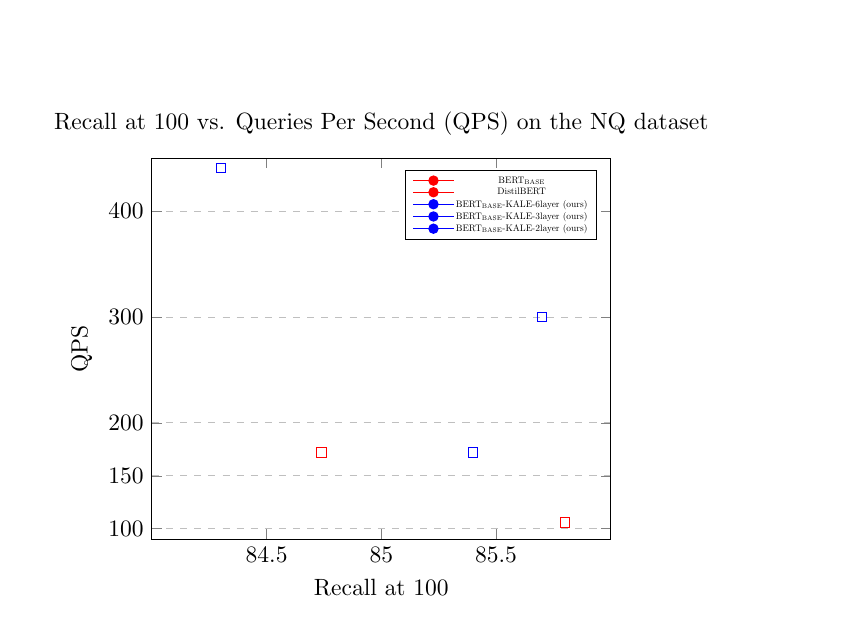
\begin{tikzpicture}
\scalebox{0.85}{
\begin{axis}[
    title={Recall at 100 vs. Queries Per Second (QPS) on the NQ dataset},
    xlabel={Recall at 100},
    ylabel={QPS},
    xmin=84, xmax=86,
    ymin=90 , ymax=450,
    xtick={84.5, 85, 85.5},
    ytick={100, 150, 200, 300,400},
    legend pos=north east,
    ymajorgrids=true,
    grid style=dashed,
    legend style={nodes={scale=0.4, transform shape}}, 
    legend image post style={mark=*}
]
\addplot[
    color=red,
    mark=square,
    ]
    coordinates {
    (85.8,106)
    };

\addplot[
    color=red,
    mark=square,
    ]
    coordinates {
    (84.74,172)
    };
\addplot[
    color=blue,
    mark=square,
    ]
    coordinates {
    (85.4,172)
    };
\addplot[
    color=blue,
    mark=square,
    ]
    coordinates {
    (85.7,300)
    };
\addplot[
    color=blue,
    mark=square,
    ]
    coordinates {
    (84.3,441)
    };

\legend{BERT\textsubscript{BASE}, DistilBERT, BERT\textsubscript{BASE}-KALE-6layer (ours),BERT\textsubscript{BASE}-KALE-3layer (ours), BERT\textsubscript{BASE}-KALE-2layer (ours) }
 \end{axis}}
\end{tikzpicture}
    \centering
    \caption{Using KALE and asymmetric training on the lead to when measuring QPS vs. Recall at 100 on the NQ dataset. Using Asymmetry and KALE, it is possible to 3x QPS with no loss in accuracy and 4.5x with 1\% loss in performance. We calculate QPS as the mean number of queries per second with a batch size of 1 and a max sequence length of 32 on a T4 GPU}
    \label{fig:speed}
\end{figure}
A bi-encoder-based retrieval, often called dense retrieval, is a retrieval function that leverages the vector representation of queries and documents as a proxy for relevance. Using two encoders, one for the query and one for the document, the input data is mapped into a common latent space where closeness becomes a proxy for relevance. \\
Dense retrievers have become increasingly popular due to their ability to capture the semantic relationships between query and document terms. However, bi-encoder-based models can also be computationally expensive, particularly when dealing with large datasets. As a result, there has been a growing interest in methods for compressing these models to reduce their computational complexity without sacrificing performance.\\
In this paper, we explore the role of asymmetry in the size of query and document encoders that leverage language models. Through experiments on several benchmarks, we demonstrate that our approach can significantly reduce the number of parameters in the bi-encoder model without sacrificing performance. \\
As shown in figure \ref{fig:speed}, the combination of asymmetric bi-encoders and post-training KALE allows for 3x more QPS than an uncompressed bi-encoder with less than 1\% loss in accuracy and nearly 5x with less than 2\%.    \\
Building on the favorable implications of asymmetry for efficient inference, we introduce a compression mechanism called \textbf{K}ullback-Leibler \textbf{Al}lingment of \textbf{E}mbeddings (KALE). KALE uses a divergence-based alignment of representations to compress models without requiring any form of retraining or index regeneration. \\
To ground our approaches, we evaluate the effectiveness of KALE and asymmetry on several benchmark datasets and compare the results to existing efficient inference approaches. \\
The following research questions drive our work: 
\begin{itemize}
    \item Is the performance of dense retrieval methods more driven by the query or document encoder size?
    \item Is it possible to compress query encoders without retraining and index regeneration?
    \item How can dense retrieval asymmetry and post-training alignment be leveraged to improve query encoder latency?
\end{itemize}
It is in answering these questions that we deliver the following contributions: 
\begin{itemize}
\item We present the first robust study on the role of document-query encoder symmetry, demonstrating that the size of the document encoder dominates performance. 
\item We introduce and demonstrate the effectiveness of KALE, a post-training compression and alignment approach demonstrating its effectiveness and 
\item We empirically demonstrate on various benchmarks how Asymmetric Compression can lead to 4.5 better QPS with 1\% loss in recall accuracy at 100.
\end{itemize}
\section{Related Work}
\textbf{Transformer Based Language Models} such as BERT \cite{Devlin2019BERTPO} and T5 \cite{Raffel2020ExploringTL} provide contextual language representations built on the Transformer architecture \cite{Vaswani2017AttentionIA} which can be specialized and adapted for specific tasks and domains \cite{Lee2020BioBERTAP}. Using these models, it becomes relatively easy to excel at a broad range of natural languages processing tasks such as question answering, text classification, and sentiment analysis. \\
\begin{table*}[htb!]
    \centering
    \caption{Information about the architecture and attributes of the FLAN-T5 models}
    \scalebox{0.62}{
    \begin{tabular}{|l|l|l|l|l|l|l|l|l|l|}
    \hline
        Model & Size(MBs) & Parameters & Encoder Layers & Parameters Encoder & Decoder Layers & Parameters decoder & Ratio End:Dec & Hidden Size \\ \hline
        Flan-t5-small \footnote{https://huggingface.co/google/flan-t5-small} & 146 & 60511616 & 8 & 35332800 & 8 & 41628352 & 0.849 & 512 \\ \hline
        Flan-t5-base \footnote{https://huggingface.co/google/flan-t5-base} & 472 & 222903552 & 12 & 109628544 & 12 & 137949312 & 0.795 & 768 \\ \hline
        Flan-t5-large \footnote{https://huggingface.co/google/flan-t5-large} & 1500 & 750251008 & 24 & 341231104 & 24 & 441918976 & 0.772 & 1024 \\ \hline
    \end{tabular}}
    \label{tab:models}
\end{table*}
\textbf{Scaling Laws} has become an increasingly important area of study as models' size and training data grows. Performance of the transformer-based language model improves with the relation to model size \cite{Radford2018ImprovingLU} and that larger models outperform smaller models \cite{Brown2020LanguageMA} on most NLP tasks. Increasing the training corpus size can lead to large improvements in performance, and model sizes can have a \textit{optimal} training data size \cite{Hoffmann2022TrainingCL}. Li et al. (2020) \cite{Li2020TrainLT} explore the relationship between model size and training efficiency finding larger models train faster and are more robust to pruning and quantization \cite{Na2022TrainFT}. \\
Rosenfeld et al. 2020 demonstrate that unstructured pruning impacts follow scaling laws \cite{Rosenfeld2020OnTP} where larger models can be pruned with greater ease. Despite this broad study of scaling laws, to our knowledge, we have not found any research focusing on the scaling laws of sequence-to-sequence models for summarization tasks. \\
\textbf{Asymmetrical in sequence-to-sequence models} broadly refers to non-uniformity between encoder and decoder model shape or attributes. Training and inference procedures should match as closely as possible \cite{Ranzato2015SequenceLT} \cite{Mihaylova2019ScheduledSF} as improvements in training loss during optimization result in improvements in model performance during Inference. While this may lead to the best model performance, it ignores the variable inference cost of models sequence to sequence models.  \\
During Inference, latency is dominated by the asymmetric execution of the language model. The auto-encoding encoder executes once over the entire input sequence, while the auto-regressive decoder executes iteratively until an end-of-sequence token is produced. \\
Kasai et al. demonstrated how the sequence-to-sequence language model performance for machine translation is dominated by the encoder depth \cite{Kasai2020DeepES}. Tay et al. 2021 extend this work by finding a \textit{DeepNarrow} which shows that for broad language modeling, it is possible to have 50\% fewer parameters and a 40\% faster inference with no loss in accuracy \cite{Tay2021ScaleEI}. \\
\textbf{Efficient Inference} for language modeling is a growing area of study that broadly focuses on reducing the inference cost without losses in accuracy. \\
Unstructured Pruning has been broadly studied \cite{Han2015ADN}  \cite{Sanh2020MovementPA} \cite{Kurti2022TheOB} \cite{Zafrir2021PruneOF} \cite{Campos2022SparseBERTSM} but realizing speedups can be difficult. \\ Structured Pruning removes fundamental structural components in a language model such as individual attention heads \cite{Voita2019AnalyzingMS} or entire model layers such as transformer encoders \cite{sanh2019distilbert}. \\
\textbf{Compressing Sequence-to-sequence} is a growing area of study where approaches from regular, efficient Inference has shown some transfer ability. Shleifer et al. show that it is possible to gain 1.93x speedup on a BART summarization model by applying structural pruning \cite{Shleifer2020PretrainedSD} but find compression approaches differ in their success depending on the dataset. Leveraging semi-structured pruning, Lagunas et al. can gain a 1.19 speedup \cite{Lagunas2021BlockPF} for minor losses in accuracy. While they find that the encoder is easier to prune than the decoder, they do not use this evidence of asymmetry to speed up performance further. \\
Li et al. investigate how to enable quantization, finding that without specialized distillation during quantization, performance collapses \cite{Li2022DQBARTES}.
Leveraging that generation occurs iteratively, and some tokens are easier to generate than other CALM \cite{Schuster2022ConfidentAL} apply early exiting to improve inference speed by 1.4x. While existing work has found interest in asymmetry, it has not been studied directly, nor has relationships in model scale been explored. \\
While there are other approaches such as knowledge distillation \cite{Hinton2015DistillingTK} \cite{sanh2019distilbert} \cite{Jiao2020TinyBERTDB}, quantization \cite{Zafrir2019Q8BERTQ8}, early exiting \cite{Xin2020DeeBERTDE} and token pruning \cite{Kim2021LearnedTP} these are not the focus on our work. 
\section{Method}
While quantization and pruning have been well studied as applied to language models, work has studied the compression BERT\textsubscript{base} or BERT\textsubscript{large}. Despite existing research, we find that a clear case study that explores how best to create a family of compressed models is lacking, and this work seeks to remedy that. As part of our research, we compare the impact of varying pruning methods, pruning stage, teachers for KD, and freezing portions of the model as applied to the RoBERTa language model.\\
While performing task-specific compression allows NLP practitioners to broadly adopt improvements in inference efficiency, having access to pre-optimized models is key. We produce a family of 8 general purpose language models, collectively called oBERTa, which progressively get smaller and faster with minimal losses in accuracy. \\
The oBERTa models leverage a combination of structured and unstructured pruning to provide a set of compressed models which can meet a wide set of latency needs. This compression approach has not been extensively documented nor discussed. Our approach to producing the oBERTA models builds on prior explorations of the combination of compression methods \cite{Kurti2022TheOB} and addresses compression approaches in a staged manner as shown in Figure~\ref{fig:framework}.\\
First, we create three structural variants starting with a RoBERTa\textsubscript{base} model. The base uses 12 transformer layers, the medium uses 6, and the small uses 3. Following prior work, we select interleaved layers for the 6-layer model and the first, middle, and last layers for the 3-layer model. Then, each of these 3 models is further pre-trained using masked language modeling on the Wikipedia-Bookcorpus text dataset, leveraging KD from a  RoBERTa\textsubscript{large} teacher. After that, each model is pruned using gradual magnitude pruning (GMP) to a desired sparsity level (90\% and 95\%) during additional pre-training based on masked language modeling, similar to Zafir et al. \cite{Zafrir2021PruneOF}. Further background on the RoBERTA model and why we did not prune using the WebText corpus can be found in the appendix. \\
After pre-training, the sparsity profile is fixed, and models are fine-tuned and quantized on their target task with a small set of variable hyperparameters. Experimentation on the impact of larger teachers, frozen embeddings, and variations in pruning algorithms are discussed in subsequent portions of this work. 
\subsection{Downstream Compression}
We explore the impact of introducing unstructured sparsity during task-specific fine-tuning. We repeat each experiment with three different seeds and report the average F1 and Exact Match (EM) metrics in tables ~\ref{tab:OBS-downstream-squad} and \ref{tab:gmp-downstream-squad}. Following a basic hyperparameter sweep, our baseline RoBERTa\textsubscript{base} model achieves a performance of 83.95 EM and 91.13 F1 in the broadly used question-answering benchmark SQUAD V1.1 \cite{Rajpurkar2016SQuAD10}. \\
We also perform unstructured pruning varying the sparsity 50-95\% and the pruning method: GMP and OBS. We prune each model for eight epochs, followed by an additional two epochs to allow the network to stabilize and re-converge. Knowledge distillation is used during training with the dense baseline model as a teacher, hardness set to $1.0$ and temperature set to $5.0$.  Further hyperparameters are in the appendix \ref{sec:downstream}.\\
Table \ref{tab:Sparse-Benchmark} shows the impact of sparsity on BERT\textsubscript{base}, as reported by previous work. Comparing these results with tables \ref{tab:OBS-downstream-squad} and \ref{tab:gmp-downstream-squad}, we conclude that RoBERTa is more sensitive to pruning than BERT, although RoBERTa\textsubscript{base} pruned with OBS remains significantly more accurate than BERT\textsubscript{base} for the same level of sparsity.\\
Table~\ref{tab:OBS-downstream-squad} shows that pruning RoBERTA\textsubscript{base} to 90\% with OBS results in a relative drop in F1 of 1.59\%, which is three times the relative drop reported for BERT\textsubscript{base} with the same pruning algorithm.
Moreover, table~\ref{tab:gmp-downstream-squad} shows that RoBERTA\textsubscript{base} becomes very sensitive to pruning with GMP for sparsities above 85\%, with the relative drop in F1 increasing almost threefold between 85\% and 90\% sparsity.
We conjecture that RoBERTa is more sensitive to pruning than BERT because the latter is relatively under-trained \cite{Liu2019RoBERTaAR}, making the more optimized RoBERTa more sensitive to the loss in expressivity caused by pruning.
\begin{table}[!ht]
    \centering
    \tiny
    \begin{tabular}{|l|l|l|l|}
    \hline
        Model & Sparsity& F1& Impact  \\ \hline
         BERT\textsubscript{base} \cite{Devlin2019BERTPO} & 0 & 88.50 & N/A \\ \hline
         BERT\textsubscript{large} \cite{Devlin2019BERTPO} & 0 &  90.9 & N/A \\ \hline
         RoBERTa\textsubscript{base} \cite{Liu2019RoBERTaAR} & 0 & 91.13 & N/A \\ \hline
         RoBERTA\textsubscript{large} \cite{Liu2019RoBERTaAR} & 0 & 94.60 & N/A \\ \hline
         PruneBert\textsubscript{base} \cite{Sanh2020MovementPA} & 90 & 84.90 & -4.07 \%\\ \hline
         PruneOFA\textsubscript{large} \cite{Zafrir2021PruneOF}& 90 & 87.25 & -1.41 \% \\ \hline
         oBERT\textsubscript{large} \cite{Kurti2022TheOB} & 90 & 87.98 &  -0.58\%  \\ \hline
         $GMP_\star$\textsubscript{large} \cite{Kurtic2022GMPWG} & 90 & 86.7 & -2.03\% \\ \hline
    \end{tabular}
    \caption{Performance of existing dense and sparse language models on the SQUAD v1.1 Question Answering Dataset}
    \label{tab:Sparse-Benchmark}
\end{table}
\begin{table}[!ht]
    \centering
    \small
    \begin{tabular}{|l|l|l|l|l|}
    \hline
        Sparsity (\%) & EM & Impact & F1 & Impact \\ \hline
        50 & 84.80 & 1.01\% & 91.49 & 0.40\% \\ \hline
        60 & 84.64 & 0.82\% & 91.33 & 0.22\% \\ \hline
        70 & 84.42 & 0.56\% & 91.13 & 0.00\% \\ \hline
        80 & 84.64 & 0.82\% & 91.33 & 0.22\% \\ \hline
        85 & 82.89 & -1.26\% & 90.12 & -1.11\% \\ \hline
        90 & 82.48 & -1.75\% & 89.68 & -1.59\% \\ \hline
        95 & 79.01 & -5.89\% & 87.05 & -4.47\% \\ \hline
    \end{tabular}
    \caption{Impact of Sparsity introduced by OBS on the F1 and EM scores of pruned RoBERTa models on the SQUAD V1.1 Dataset}
    \label{tab:OBS-downstream-squad}
\end{table}

\begin{table}[!ht]
    \centering
    \small
    \begin{tabular}{|l|l|l|l|l|}
    \hline
        Sparsity (\%) & EM & Impact & F1 & Impact \\ \hline
        50 & 84.90 & 1.13\% & 91.46 & 0.36\% \\ \hline
        60 & 84.27 & 0.38\% & 90.91 & -0.24\% \\ \hline
        70 & 83.37 & -0.69\% & 90.30 & -0.91\% \\ \hline
        80 & 81.64 & -2.76\% & 88.86 & -2.49\% \\ \hline
        85 & 81.64 & -2.76\% & 88.86 & -2.49\% \\ \hline
        90 & 76.51 & -8.86\% & 84.90 & -6.83\% \\ \hline
        95 & 69.39 & -17.34\% & 79.35 & -12.93\% \\ \hline
    \end{tabular}
    \caption{Impact of Sparsity introduced by GMP on the F1 and EM scores of pruned RoBERTa models on the SQUAD V1.1 Dataset}
    \label{tab:gmp-downstream-squad}
\end{table}
\subsection{Upstream Compression}
Based on our fine-tuning experiments, achieving a high degree of sparsity on the RoBERTA model leads to improvements in performance, but there are greater than expected losses in accuracy. Additionally, such compression is task-specific and non-amortizable, so we explore how best to generate general pruned RoBERTa models. While we eventually apply the winning set of training combinations to all of our variants of oBERTa, we first seek to answer the following questions: Does GMP or OBS perform better during pretraining pruning? Does Freezing the Embeddings during pretraining pruning further improve performance? Does the use of larger teachers further improve performance? \\
We prune various models while varying individual variables during pretraining to evaluate these questions. We experiment by pruning an oBERTa\textsubscript{base} (12 layers) model to 90\% and 95\% sparsity on all non-embedding layers. All pretraining pruning happens using the Wikipedia-BookCorpus dataset, where we train for five epochs using a learning rate of 5e-5 and a batch size of 256 using 4 A100 GPUS. To evaluate the impact of these models, we evaluate performance on the previously used SQUAD v1.1 question-answering dataset, where we train with a fixed training regime of 10 epochs with a learning rate of 1.5e-4 based on the work of Kurtic et al. We train without KD for each finetuning run with an unpruned RoBERTa\textsubscript{base} or an unpruned RoBERTa\textsubscript{large}. Details for the hyperparameters used to train all teacher models can be found in the appendix \ref{sec:TeacherStats}.  \\
\begin{table}[!ht]
    \centering
    \tiny
    \scalebox{0.65}{
    \begin{tabular}{|l|*4l|*4l|}
    \toprule
         &  \multicolumn{4}{l}{GMP} & \multicolumn{4}{l}{OBS} \\ 
        \toprule
        Model & F1 & Impact & EM & Impact & F1 & Impact & EM & Impact \\ \hline
        RoBERTA\textsubscript{base} & 92.18 & 0.00\% & 85.59 & 0.00\% & 92.18 & 0.00\% & 85.59 & 0.00\% \\ \hline
        oBERTa 90\% No KD & 88.34 & -4.17\% & 80.19 & -6.31\% & 87.72 & -4.83\% & 79.35 & -7.29\% \\ \hline
        oBERTa 90\% RoBERTA\textsubscript{base} KD & 88.75 & -3.72\% & 81.35 & -4.95\% & 88.60 & -3.88\% & 81.37 & -4.93\% \\ \hline
        oBERTa 90\% RoBERTA\textsubscript{large} KD & 89.65 & -2.75\% & 83.12 & -2.88\% & 89.63 & -2.76\% & 82.94 & -3.09\% \\ \hline
        oBERTa 95\% No KD & 86.58 & -6.07\% & 78.81 & -7.92\% & 84.90 & -7.90\% & 76.82 & -10.25\% \\ \hline
        oBERTa 95\% RoBERTA\textsubscript{base} KD & 86.99 & -5.63\% & 79.41 & -7.22\% & 86.14 & -6.55\% & 78.63 & -8.13\% \\ \hline
        oBERTa 95\% RoBERTA\textsubscript{large} KD & 87.60 & -4.97\% & 80.44 & -6.01\% & 86.14 & -6.55\% & 79.84 & -6.72\% \\ \hline
        \bottomrule
    \end{tabular}}
    \caption{Impact on F1 of SQUAD V1.1 of using OBS vs. GMP as the pruning method during pretraining. Impact measures the relative loss in performance vs. the unpruned RoBERTa\textsubscript{base} baseline.}
    \label{tab:OBS-vs-GMP-hard1.0}
\end{table}
Comparing the use of OBS vs. GMP as shown in table \ref{tab:OBS-vs-GMP-hard1.0}, we can see that GMP consistently outperforms OBS. This is the opposite of what is seen when pruning downstream or, in prior work, pruning BERT. We attribute this inversion to not using the web-text dataset and leveraging the Wikipedia-book-corpus instead. We believe that without access to the original training corpus OBS is leading to overfitting of the sparse models, a dataset that is not its intended target. \\
\begin{table}[!ht]
    \centering
    \small
    \scalebox{0.57}{
    \begin{tabular}{|l|*4l|*4l|}
    \toprule
         &  \multicolumn{4}{l}{Hardness 0.5} & \multicolumn{4}{l}{Hardness 1.0} \\ 
        \toprule
        Model & F1 & Impact & EM & Impact & F1 & Impact & EM & Impact \\ \hline
         RoBERTA\textsubscript{base} & 92.18 & 0.00\% & 85.59 & 0.00\% & 92.18 & 0.00\% & 85.59 & 0.00\% \\ \hline
        oBERTa 90\% No KD & 88.21 & -4.31\% & 80.19 & -6.31\% & 88.34 & -4.17\% & 80.19 & -6.31\% \\ \hline
        oBERTa 90\% Base KD & 89.19 & -3.25\% & 81.74 & -4.50\% & 88.75 & -3.72\% & 81.35 & -4.95\% \\ \hline
        oBERTa 90\% Large KD & 90.14 & -2.21\% & 83.51 & -2.43\% & 89.65 & -2.75\% & 83.12 & -2.88\% \\ \hline
        oBERTa-95 No KD & 85.82 & -6.90\% & 77.77 & -9.14\% & 86.58 & -6.07\% & 78.81 & -7.92\% \\ \hline
        oBERTa-95 Base KD & 86.98 & -5.64\% & 79.23 & -7.43\% & 86.99 & -5.63\% & 79.41 & -7.22\% \\ \hline
        oBERTa-95 Large KD & 87.66 & -4.91\% & 80.40 & -6.07\% & 87.60 & -4.97\% & 80.44 & -6.01\% \\ \hline
        \bottomrule
    \end{tabular}}
    \caption{Impact on F1 of SQUAD V1.1 by hardness in KD during pretraining pruning. Impact measures the relative loss in performance vs. the unpruned RoBERTa\textsubscript{base} baseline.}
    \label{tab:hardness-oberta}
\end{table}
  Evaluating the impact of variations in the hardness  of KD as shown in table \ref{tab:hardness-oberta}, there is a bit more of a muted set of conclusions. The 95\% sparse models perform better with a hardness of 1.0, while the 90\% models do better with a hardness of 0.5. Given that our goal is to preserve most of the RoBERTa model without actually using its large dataset, we set our hardness to 1.0 as it keeps the model from explicitly learning the new dataset. \\
\begin{table}[!ht]
    \centering
    \small
    \scalebox{0.5}{
    \begin{tabular}{|l|*4l|*4l|}
    \toprule
          &  \multicolumn{4}{l}{Frozen Embeddings} & \multicolumn{4}{l}{Trained Embeddings} \\ 
        \midrule
        Model & F1 & Impact & EM & Impact & F1 & Impact & EM & Impact \\ \hline
        RoBERTa\textsubscript{base} & 92.18 & 0.00\% & 85.59 & 0.00\% & 92.18 & 0.00\% & 85.59 & 0.00\% \\ \hline
        oBERTa\textsubscript{base} 90\% no KD & 87.71 & -4.85\% & 79.62 & -6.98\% & 88.21 & -4.31\% & 80.19 & -6.31\% \\ \hline
        oBERTa\textsubscript{base} 90\% RoBERTa\textsubscript{base} KD & 89.7 & -2.69\% & 81.74 & -4.50\% & 89.19 & -3.24\% & 83.07 & -2.94\% \\ \hline
        oBERTa\textsubscript{base} 90\% RoBERTa\textsubscript{large} KD & 89.59 & -2.81\% & 82.98 & -3.05\% & 90.14 & -2.21\% & 83.51 & -2.43\% \\ \hline
        \bottomrule
    \end{tabular}}
    \caption{Impact on F1 of SQUAD V1.1 with respect to the use of frozen embeddings or not during pretraining pruning. Impact measures the relative loss in performance vs. the unpruned RoBERTa\textsubscript{base} baseline.}
    \label{tab:freeze-embd-oberta}
\end{table}
When we evaluate the impact of freezing embeddings during pre-training, as shown in table \ref{tab:freeze-embd-oberta}, we find strong evidence that using frozen embeddings consistently leads to worse performance and, as a result, does not freeze embeddings during our model pruning. Looking at the impact of varying the size of the teacher for pretraining KD as shown in table \ref{tab:upsteam-teach}, we unsurprisingly find clear evidence that using a larger teacher during pretraining pruning leads to improvements in performance. \\
\begin{table}[!ht]
    \centering
    \small
    \scalebox{0.55}{
    \begin{tabular}{|l|*4l|*4l|}
    \toprule
          &  \multicolumn{4}{l}{Base Upstream Teacher} & \multicolumn{4}{l}{Large Upstream Teacher} \\ 
        \midrule
        Model & F1 & Impact & EM & Impact & F1 & Impact & EM & Impact \\ \hline
        RoBERTA\textsubscript{base} & 92.18 & 0.00\% & 85.59 & 0.00\% & 92.18 & 0.00\% & 85.59 & 0.00\% \\ \hline
        oBERTa 90\% no KD  & 88.34 & -4.17\% & 80.59 & -5.84\% & 88.1 & -4.43\% & 80.06 & -6.46\% \\ \hline
        oBERTa 90\% Base KD & 88.75 & -3.72\% & 81.35 & -4.95\% & 89.22 & -3.21\% & 82.02 & -4.17\% \\ \hline
        oBERTa 90\% Large KD & 89.65 & -2.74\% & 83.12 & -2.89\% & 89.98 & -2.39\% & 83.14 & -2.86\% \\ \hline
        \bottomrule
    \end{tabular}}
    
    \caption{Impact on F1 of SQUAD V1.1 with respect variation is the size of the teacher in KD during pretraining pruning. Impact measures the relative loss in performance vs. the unpruned RoBERTa\textsubscript{base} baseline.}
    \label{tab:upsteam-teach}
\end{table}
Using these experiments, we generate the recipe, which we then use to create the many variants of oBERTa. We pre-train models using KD using a RoBERTa\textsubscript{large} teacher with a hardness of 1.0; we do not freeze the embeddings and use GMP to prune.
\section{KL Alignment of Embeddings}
Based on the aforementioned experiments, we generate 8 variants of oBERTa, each with a different size and sparsity profile; details can be found in table \ref{tab:oberta-model-info}. Within this table, we report the impact on the model size as measured by the raw and compressed size of the ONNX \footnote{https://onnx.ai/} model file. Embeddings are unpruned and each layer is pruned to the target sparsity profile independent of the rest of the model. As a result, the overall sparsity profile may vary as modules in the network may not be able to reach exactly 90\% or 95\% sparsity. \\
Using these \textit {inference-optimized} models, we evaluate their \textit{sparse transfer} performance by finetuning these models on their target task using a fixed training regime and minor hyperparameter exploration. For each task, we train them for 10 epochs or 20 (10 of which are Quantization Aware Training), with the longer schedule being reserved for models which are being quantized.  \\
We evaluate performance on a benchmark of diverse NLP tasks ranging from question answering, sentiment analysis, document classification, token classification, and text classification. For question answering, we leverage the SQuAD v1.1 \cite{Rajpurkar2016SQuAD10} and SQuAD V2.0 \cite{Rajpurkar2018KnowWY} datasets. We leverage the SST-2 \cite{socher-etal-2013-recursive} dataset for sentiment analysis. For text classification, we use the Quora Duplicate Query Detection (QQP) \cite{sambitsekhar_2017} and the MNLI \cite{N18-1101} datasets. We leverage the IMDB \cite{maas-EtAl:2011:ACL-HLT2011} dataset for document classification and CONLL2003 \cite{tjong-kim-sang-de-meulder-2003-introduction} for token classification.\\ 
Looking at performance on question answering as shown in table \ref{tab:sparse-transfer-squad} and \ref{tab:sparse-transfer-squad2}.
\begin{table}[!ht]
    \centering
    \tiny
    \scalebox{0.8}{
    \begin{tabular}{|l|*3l|*3l|}
    \toprule
         &  \multicolumn{3}{l}{Sparse Transfer} & \multicolumn{3}{l}{Sparse Transfer With Quantization} \\ 
        \midrule
        model & F1 & Recovery & EM & F1 & Recovery & EM \\ \hline
        oBERTa\textsubscript{base} & 92.15 & 100.00\% & 85.78 & 93.18 & 101.11\% & 87.29 \\ \hline
        oBERTa\textsubscript{base} 90$\backslash$\% & 90.95 & 98.69\% & 84.42 & 89.46 & 97.08\% & 82.61 \\ \hline
        oBERTa\textsubscript{base} 95$\backslash$\% & 89.84 & 97.49\% & 83.08 & 89.23 & 96.83\% &  81.12\\ \hline
        oBERTa\textsubscript{MEDIUM} & 90.37 & 98.06\% & 83.84 & 83.77 & 90.91\% & 90.37 \\ \hline
        oBERTa\textsubscript{MEDIUM} 90$\backslash$\% & 89.26 & 96.86\% & 82.18 & 88.65 & 96.20\% & 81.88 \\ \hline
        oBERTa\textsubscript{SMALL} & 84.87 & 92.09\% & 76.55 & 84.82 & 92.05\% & 76.77 \\ \hline
        oBERTa\textsubscript{SMALL} 90$\backslash$\% & 84.66 & 91.87\% & 76.18 & 82.18 & 92.18\% & 74.21\\ 
        \bottomrule
    \end{tabular}}
   
    \caption{Sparse Transfer performance of the oBERTA family on the SQUAD V1.1 dataset. The sparse transfer was performed over 10 epochs and sparse transfer with quantization over 20. Recovery is based on the relative performance of the unpruned oBERTa\textsubscript{base}. }
    \label{tab:sparse-transfer-squad}
\end{table}
\begin{table}[!ht]
    \centering
    \begin{tiny}
    \scalebox{0.8}{
    \begin{tabular}{|l|*3l|*3l|}
    \toprule
         &  \multicolumn{3}{l}{Sparse Transfer} & \multicolumn{3}{l}{Sparse Transfer With Quantization} \\ 
        \midrule
         model & F1 & Recovery & EM & F1 & Recovery & EM \\ \hline
        oBERTa\textsubscript{base} & 82.77 & 100.00\% & 79.56 & 85.298 & 103.06\% & 82.347 \\ \hline
        oBERTa\textsubscript{base} 90$\backslash$\% & 81.33 & 98.26\% & 78.27 & 81.43 & 98.38\% & 78.92 \\ \hline
        oBERTa\textsubscript{base} 95$\backslash$\% & 77.98 & 94.22\% & 74.67 & 78.09 & 94.35\% & 74.82 \\ \hline
        oBERTa\textsubscript{MEDIUM} & 77.51 & 93.65\% & 74.25 & 78.137 & 94.41\% & 75.179 \\ \hline
        oBERTa\textsubscript{MEDIUM} 90$\backslash$\% & 76.64 & 92.60\% & 73.34 & 76.24 & 92.11\% & 73.51 \\ \hline
        oBERTa\textsubscript{SMALL} & 71.54 & 86.44\% & 67.93 & 71.591 & 86.50\% & 68.087 \\ \hline
        oBERTa\textsubscript{SMALL} 90$\backslash$\% & 70.79 & 85.53\% & 67.31 & 69.35 & 87.79\% & 65.21 \\ \hline
        \bottomrule
    \end{tabular}}
    \end{tiny}
    \caption{Sparse Transfer performance of the oBERTA family on the SQUAD V2.0 dataset. The sparse transfer was performed over 10 epochs, and sparse transfer with quantization over 20. Recovery is based on the relative performance of the unpruned oBERTa\textsubscript{base}. }
    \label{tab:sparse-transfer-squad2}
\end{table}
Moving to text classification on QQP and MNLI as shown in tables \ref{tab:sparse-transfer-qqp} and \ref{tab:sparse-transfer-MNLI}
\begin{table}[!ht]
    \centering
    \begin{tiny}
    \scalebox{0.70}{
    \begin{tabular}{|l|*3l|*3l|}
    \toprule
         &  \multicolumn{3}{l}{Sparse Transfer} & \multicolumn{3}{l}{Sparse Transfer With Quantization} \\ 
        \midrule
         model & Accuracy & Recovery &Accuracy(MM) & Accuracy & Recovery & Accuracy(MM) \\ \hline
        oBERTa\textsubscript{base} & 87.88\% & 100.00\% & 87.57\% & 88.06\% & 100.20\% & 88.01\% \\ \hline
        oBERTa\textsubscript{base} 90\% & 85.17\% & 96.91\% & 84.73\% & 85.09\% & 96.83\% & 84.76\% \\ \hline
        oBERTa\textsubscript{base} 95\% & 84.32\% & 95.95\% & 84.08\% & 83.73\% & 95.28\% & 83.83\% \\ \hline
        oBERTa\textsubscript{MEDIUM} & 85.29\% & 97.05\% & 85.17\% & 83.62\% & 95.15\% & 83.74\% \\ \hline
        oBERTa\textsubscript{MEDIUM} 90\% & 81.61\% & 92.87\% & 81.32\% & 82.37\% & 93.73\% & 81.79\% \\ \hline
        oBERTa\textsubscript{SMALL} & 80.80\% & 91.95\% & 81.55\% & 81.10\% & 92.29\% & 81.51\% \\ \hline
        oBERTa\textsubscript{SMALL} 90\% & 79.23\% & 90.15\% & 79.24\% & 79.14\% & 90.06\% & 79.42\% \\ \hline
        \bottomrule
    \end{tabular}}
    \end{tiny}
    \caption{Sparse Transfer performance of the oBERTA family on the MNLI dataset. Sparse transfer was performed over 10 epochs and sparse transfer with quantization over 20. Recovery is based on the relative performance of the unpruned oBERTa\textsubscript{base}. }
    \label{tab:sparse-transfer-MNLI}
\end{table}
\begin{table}[!ht]
    \centering
    \begin{tiny}
    \scalebox{0.6}{
    \begin{tabular}{|l|*4l|*4l|}
    \toprule
         &  \multicolumn{4}{l}{Sparse Transfer} & \multicolumn{4}{l}{Sparse Transfer With Quantization} \\ 
        \midrule
        model & Accuracy & Recovery & F1 & Combined & Accuracy & Recovery & F1 & Combined \\ \hline
        oBERTa\textsubscript{base} & 91.52\% & 100.00\% & 90.09\% & 88.66\% & 89.86\% & 98.18\% & 88.12\% & 86.73\% \\ \hline
        oBERTa\textsubscript{base} 90\% & 91.01\% & 99.44\% & 89.47\% & 87.92\% & 91.21\% & 99.66\% & 89.68\% & 88.16\% \\ \hline
        oBERTa\textsubscript{base} 95\% & 90.85\% & 99.26\% & 89.21\% & 87.58\% & 90.72\% & 99.12\% & 89.08\% & 0.87\% \\ \hline
        oBERTa\textsubscript{MEDIUM} & 91.35\% & 99.81\% & 89.90\% & 88.44\% & 91.33\% & 99.79\% & 89.80\% & 88.28\% \\ \hline
        oBERTa\textsubscript{MEDIUM} 90\% & 90.48\% & 98.86\% & 88.85\% & 87.21\% & 90.60\% & 99.00\% & 89.01\% & 87.42\% \\ \hline
        oBERTa\textsubscript{SMALL} & 90.72\% & 99.13\% & 89.21\% & 87.71\% & 89.74 & 98.06\% & 87.99 & 86.25 \\ \hline
        oBERTa\textsubscript{SMALL} 90\% & 89.74\% & 98.06\% & 87.99\% & 86.25\% & 89.73 & 98.04\% & 87.98 & 86.08\\
        \bottomrule
    \end{tabular}}
    \end{tiny}
    \caption{Sparse Transfer performance of the oBERTA family on the QQP dataset. The sparse transfer was performed over ten epochs, and sparse transfer with quantization over 20. Recovery is based on the relative performance of the unpruned oBERTa\textsubscript{base}.}
    \label{tab:sparse-transfer-qqp}
\end{table}
Shifting focus to document classification as shown in table \ref{tab:sparse-transfer-imdb} and sentiment analysis in \ref{tab:sparse-transfer-SST2}
\begin{table}[!ht]
    \centering
    \begin{tiny}
    \scalebox{0.95}{
    \begin{tabular}{|l|*2l|*2l|}
    \toprule
         &  \multicolumn{2}{l}{Sparse Transfer} & \multicolumn{2}{l}{Sparse Transfer With Quantization} \\ 
        \midrule
        model & Accuracy & Recovery & Accuracy & Recovery \\ \hline
        oBERTa\textsubscript{base} & 95.24\% & 100.00\% & 95.44\% & 100.21\% \\ \hline
        oBERTa\textsubscript{base} 90\% & 93.64\% & 98.32\% & 93.28 & 97.94\% \\ \hline
        oBERTa\textsubscript{base} 95\% & 93.48\% & 98.15\% & 92.80& 97.23\% \\ \hline
        oBERTa\textsubscript{MEDIUM} & 93.36\% & 98.03\% & 94.08 & 98.78\% \\ \hline
        oBERTa\textsubscript{MEDIUM} 90\% & 92.24\% & 96.85\% & 92.08& 96.69\% \\ \hline
        oBERTa\textsubscript{SMALL} & 93.04\% & 97.69\% & 92.52 & 97.15\% \\ \hline
        oBERTa\textsubscript{SMALL} 90\% & 91.60\% & 96.18\% & 91.28 & 95.84\% \\
        \bottomrule
    \end{tabular}}
    \end{tiny}
    \caption{Sparse Transfer performance of the oBERTA family on the IMDB dataset. The sparse transfer was performed over ten epochs, and sparse transfer with quantization over 20. Recovery is based on the relative performance of the unpruned oBERTa\textsubscript{base}. }
    \label{tab:sparse-transfer-imdb}
\end{table}
\begin{table}[!ht]
    \centering
    \begin{tiny}
    \scalebox{0.95}{
    \begin{tabular}{|l|*2l|*2l|}
    \toprule
         &  \multicolumn{2}{l}{Sparse Transfer} & \multicolumn{2}{l}{Sparse Transfer With Quantization} \\ 
        \midrule
        model & Accuracy & Recovery & Accuracy & Recovery \\ \hline
        oBERTa\textsubscript{base} & 94.60 & 100.00\% & 92.66 & 97.95\% \\ \hline
        oBERTa\textsubscript{base} 90\% & 92.78 & 98.08\% & 92.546 & 97.83\% \\ \hline
        oBERTa\textsubscript{base} 95\% & 91.51 & 96.74\% & 91.399 & 96.62\% \\ \hline
        oBERTa\textsubscript{MEDIUM} & 92.89 & 98.19\% & 91.06 & 96.26\% \\ \hline
        oBERTa\textsubscript{MEDIUM} 90\% & 88.76 & 93.83\% & 89.91 & 95.04\% \\ \hline
        oBERTa\textsubscript{SMALL} & 90.48 & 95.64\% & 91.28 & 96.49\% \\ \hline
        oBERTa\textsubscript{SMALL} 90\% & 89.34 & 94.44\% & 88.65 & 93.71\% \\ 
        \bottomrule
    \end{tabular}}
    \end{tiny}
    \caption{Sparse Transfer performance of the oBERTA family on the SST-2 dataset. The sparse transfer was performed over ten epochs, and sparse transfer with quantization over 20. Recovery is based on the relative performance of the unpruned oBERTa\textsubscript{base}. }
    \label{tab:sparse-transfer-SST2}
\end{table}
Finally, looking at performance on token classification as shown in table \ref{tab:sparse-transfer-conll2003} 
\begin{table}[!ht]
    \centering
    \begin{tiny}
    \scalebox{0.75}{
    \begin{tabular}{|l|*3l|*3l|}
    \toprule
         &  \multicolumn{3}{l}{Sparse Transfer} & \multicolumn{3}{l}{Sparse Transfer With Quantization} \\ 
        \midrule
        model & Accuracy & Recovery & F1 & Accuracy & Recovery & F1 \\ \hline
        oBERTa\textsubscript{base} & 99.26\% & 100.00\% & 95.51\% & 99.30\% & 100.05\% & 95.98\% \\ \hline
        oBERTa\textsubscript{base} 90\% & 99.11\% & 99.85\% & 94.98\% & 99.05\% & 99.79\% & 94.51\% \\ \hline
        oBERTa\textsubscript{base} 95\% & 98.89\% & 99.63\% & 93.32\% & 98.75\% & 99.48\% & 92.61\% \\ \hline
        oBERTa\textsubscript{MEDIUM} & 99.04\% & 99.77\% & 94.39\% & 99.18\% & 99.92\% & 95.15\% \\ \hline
        oBERTa\textsubscript{MEDIUM} 90\% & 98.79\% & 99.53\% & 93.31\% & 98.73\% & 99.46\% & 92.70\% \\ \hline
        oBERTa\textsubscript{SMALL} & 99.01\% & 99.75\% & 94.00\% & 98.98\% & 99.72\% & 94.13\% \\ \hline
        oBERTa\textsubscript{SMALL} 90\% & 98.47\% & 99.20\% & 91.13\% & 98.25\% & 98.98\% & 89.79\% \\ 
        \bottomrule
    \end{tabular}}
    \end{tiny}
    \caption{Sparse Transfer performance of the oBERTA family on the CONLL-2003 dataset. The sparse transfer was performed over ten epochs, and sparse transfer with quantization over 20. Recovery is based on the relative performance of the unpruned oBERTa\textsubscript{base}. }
    \label{tab:sparse-transfer-conll2003}
\end{table}

\subsection{Inference Benchmark}
To evaluate the performance of our inference-optimized models, we benchmark performance using the popular DeepSparse library version 1.3.2 \footnote{pip install deepsparse==1.3.2} and an Intel Xeon Gold 6238R Processor. Performance is measured using models that have been \textit{sparse-transferred} to the SQuAD v1.1 dataset and exported to a standard ONNX model format. Benchmarks are run on 4 and 24 cores and a sequence length of 384 with batch sizes of 1, 16, and 64. For each model, the benchmark is run for 60 seconds with a warm-up period of 10 seconds, and we report the throughput (items per second) and the mean, median, and standard deviation per item latency. 
\begin{table}[!ht]
    \centering
    \begin{tiny}
    \scalebox{0.85}{
    \begin{tabular}{|l|*3l|*3l|}
    \toprule
         &  \multicolumn{3}{l}{24 Cores} & \multicolumn{3}{l}{4 Cores} \\ 
        \midrule
        Model & BS 1 & BS 16 & BS 64 &  BS 1 & BS 16 & BS 64 \\
        \midrule
        oBERTa\textsubscript{base} & 1.00 & 1.00 & 1.00 & 1.00 & 1.00 & 1.00 \\ \hline
        oBERTa\textsubscript{base} Quantized & 3.10 & 4.29 & 4.46 & 4.09 & 4.31 & 4.32 \\ \hline
        oBERTa\textsubscript{base} 90\% & 3.29 & 3.80 & 3.80 & 3.60 & 3.34 & 3.40 \\ \hline
        oBERTa\textsubscript{base} 90\% Quantized & 4.12 & 7.05 & 7.37 & 7.67 & 7.59 & 7.40 \\ \hline
        oBERTa\textsubscript{base} 95\% & 8.72 & 4.56 & 4.65 & 4.12 & 3.85 & 4.37 \\ \hline
        oBERTa\textsubscript{base} 95\% Quantized & 4.73 & 8.22 & 8.56 & 9.41 & 9.06 & 8.68 \\ \hline
        oBERTa\textsubscript{MEDIUM} & 1.96 & 1.99 & 1.99 & 1.96 & 1.99 & 2.02 \\ \hline
        oBERTa\textsubscript{MEDIUM} Quantized & 6.20 & 8.04 & 8.44 & 8.43 & 8.33 & 8.45 \\ \hline
        oBERTa\textsubscript{MEDIUM} 90\%   & 6.35 & 7.41 & 6.84 & 7.83 & 6.56 & 6.72 \\ \hline
        oBERTa\textsubscript{MEDIUM} 90\% Quantized  & 8.94 & 12.86 & 13.65 & 14.99 & 14.81 & 14.95 \\ \hline
        oBERTa\textsubscript{SMALL} & 3.89 & 3.96 & 3.99 & 3.95 & 3.97 & 4.03 \\ \hline
        oBERTa\textsubscript{SMALL} Quantized & 12.47 & 14.12 & 14.08 & 15.50 & 15.48 & 15.70 \\ \hline
        oBERTa\textsubscript{SMALL} 90\% & 12.22 & 14.40 & 14.67 & 14.05 & 14.19 & 14.13 \\ \hline
        oBERTa\textsubscript{SMALL} 90\% Quantized & 16.21 & 21.35 & 23.96 & 29.77 & 27.14 & 27.58 \\ \hline
        \bottomrule
    \end{tabular}}
    \end{tiny}
    \caption{Latency reduction of the oBERTa family concerning the unpruned oBERTa\textsubscript{base} as measured on 24 and 4 cores. Speedup is measured relative to the latency reduction in MS/batch, and BS refers to batch size.}
    \label{tab:inference-bench}
\end{table}
We present a set of summary statistics of relative speedup across batch sizes and inference server configurations as shown in table \ref{tab:inference-bench}. Full inference performance results can be found in the appendix. In analyzing performance, we can see that the introduction of quantization to a dense model delivers roughly a 4x speedup while quantization on sparse models is closer to 2x. With the introduction of sparsity, 90\% leads to slightly under 4x speedup, while 95\% leads to slightly over 4x. The impact of structural pruning is roughly equivalent to the size of the as a 6-layer model is two times faster than a 12-layer, and a 3-layer model is four times faster. Since these different compression forms are additive, we can see that a small (3-layer) 90\% quantized model performance is ~24x (4*4*2). Looking at the variation in a speedup by batch size and the number of cores, we can see that allocating more cores leads to a smaller gap in inference speedup, especially with small batches. From this, we extract that compression is significant when performing streaming inference (batch size 1) on smaller CPUs.  \\
Next, we go ahead and benchmark the oBERTa model performance against existing sparse-transfer models such as oBERT and PruneOFA using the models that have been published \footnote{Since the PruneBERT model is not available in the zoo, we extrapolate numbers using the performance of our oBERTa\textsubscript{base} pruned 90\% as both models feature 12 transformer encoders and 90\% sparsity.} in Neural Magic's Sparse-Zoo \footnote{https://sparsezoo.neuralmagic.com/}. We run these models using four cores and a batch size of 1 and compare their speedup (or slowdown) relative to their performance on the SQUAD v1.1 question-answering benchmark. Results can be found in table \ref{tab:inference-competitive-short} and full results in \ref{tab:inference-competitive-full}. Looking at the improvements in accuracy and inference throughput, we find the oBERTa models are 1.3 to 4 times better than models with approximately the same accuracy.  \\
\begin{table}[!ht]
    \centering
    \scalebox{0.5}{
    \begin{tabular}{|l|l|*2l|*2l|}
    \toprule
        \multicolumn{2}{l}{} &  \multicolumn{2}{l}{Vs. BERT\textsubscript{base}} & \multicolumn{2}{l}{Vs. BERT\textsubscript{large}} \\ \hline
        Model & F1 & Recovery & Speedup & Recovery & Speedup \\ \hline
        oBERTa\textsubscript{base} 90\% & 91.00 & 102.77\% & 3.57 & 100.44\% & 20.21 \\ \hline
        oBERT\textsubscript{large} 95\% Quantized & 90.21 & 101.87\% & 3.41 & 99.57\% & 19.31 \\ \hline
        \midrule
        prunedOFA\textsubscript{large} 90\% Quantized & 89.96 & 101.59\% & 2.38 & 99.29\% & 13.47 \\ \hline
        oBERTa\textsubscript{base} 90\% Quantized & 89.46 & 101.03\% & 7.62 & 98.74\% & 43.07 \\ \hline
        \midrule
        oBERTa\textsubscript{MEDIUM} 90\%   & 89.26 & 98.99\% & 7.78 & 96.75\% & 43.99 \\ \hline
        obert\textsubscript{base} 90\% Quantized & 88.00 & 99.38\% & 6.96 & 97.13\% & 39.37 \\ \hline
        \midrule
        oBERTa\textsubscript{SMALL} 90\% & 84.66 & 90.97\% & 13.95 & 88.91\% & 78.91 \\ \hline
        pruneBERT 90\% & 84.90 & 95.88\% & 3.57  & 93.71\% & 73.82 \\ \hline
        \bottomrule
    \end{tabular}}
    \caption{Speedups of the oBERTa-family compared to existing published sparse models compared to the performance of BERT\textsubscript{base} and BERT-large. Speedup measures the reduction in latency of MS/batch. oBERTa\textsubscript{base} 90\% exceeds the accuracy of oBERT\textsubscript{large} 95\% quantized despite being faster, oBERTa\textsubscript{base} 90\% quantized performs at the level of pruneOFA\textsubscript{large} 90\% Quantized despite being 3x faster, oBERTa\textsubscript{MEDIUM} 90\% can outperform oBERT\textsubscript{base} 90\% Quantized despite being 30\% faster, and oBERTa\textsubscript{SMALL} 90\% performs on par with pruneBERT 90\% despite being nearly four times faster. }
    \label{tab:inference-competitive-short}
\end{table}
Looking at the competitive results, we find that the oBERTa-* models can deliver significant gains in performance (F1) relative to speedups. The oBERTa\textsubscript{base}Pruned 90\% Quantized model achieves an undertaking that nearly matches pruneOFA-large 90\% Quantized while delivering nearly 13x faster inference. Similarly, the oBERTA\textsubscript{SMALL} 90\%  model provides similar accuracy to PruneBERT despite being over four times faster.
\textbf{CAPOT and typos} When queries have typos, CAPOT is a computationally efficient method of improving performance as the relative gap between unaltered and aligned is greatest on alterations like character deletion, keyboard character replacement, and random character replacement. We attribute this impact to the relative importance of our alignment dataset's character level alterations. Three out of the 10 methods focus on learning alignments based around minor character shifts, and as a result, the performance optimizes there to the detriment of other forms of noise. CAPOT is much less effective in improving the relevance of minor syntactic shifts such as lemmatization or stemming leading to marginal improvements over the unaltered baselines. We attribute this to the already smaller gap on syntactically altered queries, which on datasets such as TriviaQA have less than 2\% impact.\\
\textbf{CAPOT and Retrieval Set Depth} demonstrates that CAPOT, like DA, sees the highest impact when the recall set size is small. On the NQ the gap between CAPOT and the baseline at 20 is nearly 10\% which narrows to ~3\% at 200.  \\
\textbf{Limitations of contrastive alignment} While effective, contrastive alignment has a non-negligible impact on the retrieval accuracy of unaltered queries. As shown in table \ref{tab:capot-nq-20} on non-noisy queries the use of data augmentation incurs no loss in accuracy yet CAPOT incurs ~2.5\%. This is a fundamental issue because the alignment of embeddings causes minor variations in representations that have actual implications on retrieval accuracy. We believe that the use of larger datasets could such as the web search logs used by the Generic Intent Representation of query vectors \cite{Zhang2019GenericIR} could improve this.\\
\textbf{Poly Encoding} using alignment-based optimization we believe leads to novel retrieval methods which allow for fixed index, constrained optimizations tailored to specific types of noise or deficiencies in retrieval. Novel forms of noise-optimized encoders can be deployed in parallel without additional index generation. Given the prevalence of bi-encoders as candidate set generation tools, CAPOT, unlike Data Augmentation, can generate many targeted query encoder variants which share a document representation. As shown in figure \ref{fig:fig2}, instead of seeking a single query encoder that learns all surface and semantic forms of query representations, alignment approaches can be used to create many encoders which are tuned to various goals. 
\label{app:poly-encoder}
\begin{figure}[htb!]
    \centering
    \scalebox{0.22}{
    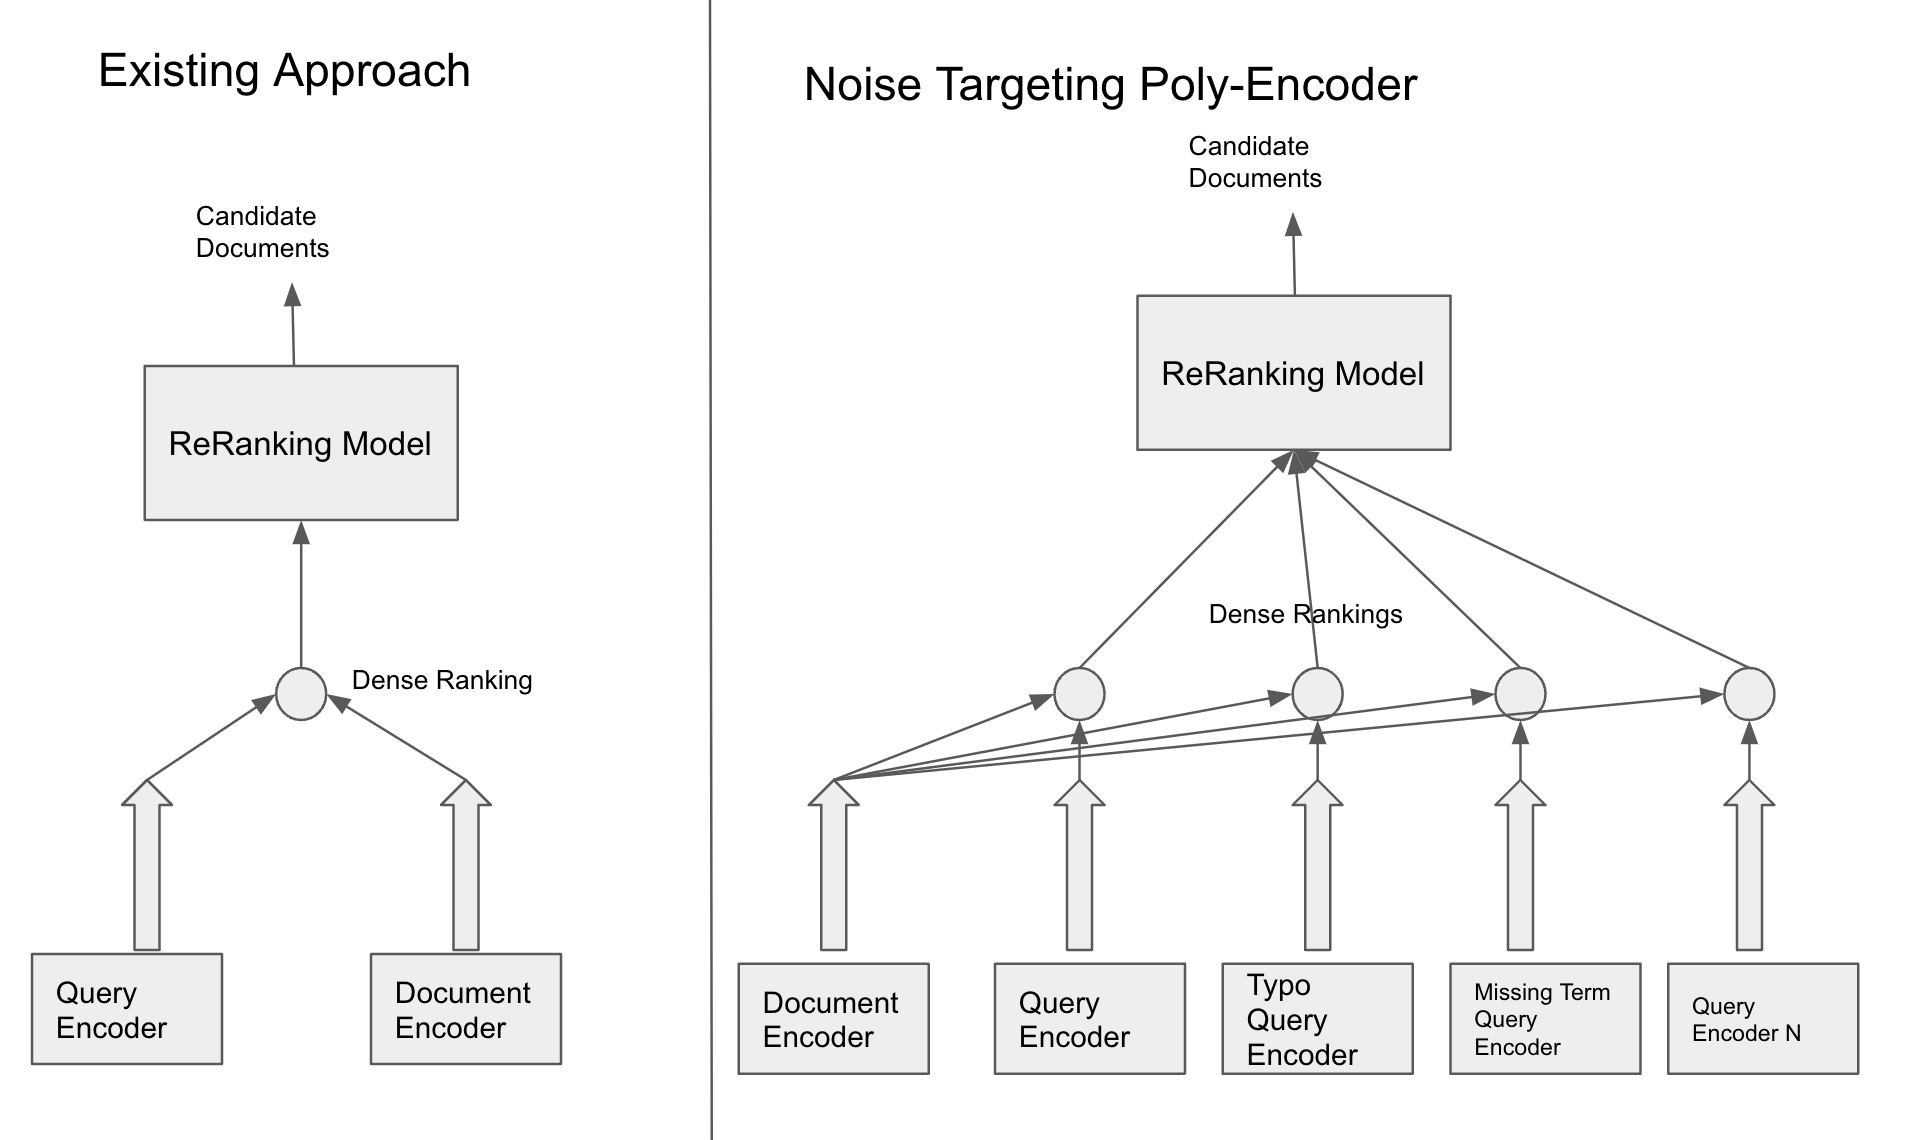
\includegraphics{figure2.png}}
    \caption{Proposed poly-encoder architecture using noise-targeted query encoders optimized with CAPOT}
    \label{fig:fig2}
\end{figure}
\bibliographystyle{acl_natbib}
\bibliography{anthology,custom}
\appendix
\section{Introducing and Transferring Sparsity for efficient inference}
\label{app:sparsity}
\section{Robust and Efficient Semantic Retrieval}
\label{app:retrieval}

\section{Scaling Multi-Lingual Classification and Abstractive Summarization to Web-Scale workloads}
\label{app:scaling-workload}

\section{Publications}
\begin{itemize}
\item \href{https://arxiv.org/abs/2203.07259}{The Optimal BERT Surgeon: Scalable and Accurate Second-Order Pruning for Large Language Models} - Eldar Kurtic, \textbf{Daniel Campos}, Tuan Nguyen, Elias Frantar, Mark Kurtz, Benjamin Fineran, Michael Goin, Dan Alistarh - \href{https://2022.emnlp.org/}{EMNLP 2022}
\item \href{https://arxiv.org/abs/2205.12452}{Sparse*BERT: Sparse Models Generalize To New tasks and Domains} - \textbf{Daniel Campos}, Alexandre Marques, Tuan Nguyen, Mark Kurtz, ChengXiang Zhai - \href{https://www.sparseneural.net/}{Sparsity in Neural Networks Workshop at ICML 2022}
\item \href{https://arxiv.org/abs/2303.17612}{oBERTa: Improving Sparse Transfer Learning via improved initialization, distillation, and pruning regimes} - \textbf{Daniel Campos}, Alexandre Marques, Mark Kurtz, ChengXiang Zhai 
\item \href{https://arxiv.org/abs/2304.00114}{Dense Sparse Retrieval: Using Sparse Language Models for Inference Efficient Dense Retrieval} - \textbf{Daniel Campos}, ChengXiang Zhai
\item \href{https://arxiv.org/abs/2304.03401}{Noise-Robust Dense Retrieval via Contrastive Alignment Post Training} - \textbf{Daniel Campos}, Alessandro Magnani, ChengXiang Zhai
\item \href{https://arxiv.org/abs/2304.01016}{Quick Dense Retrievers Consume KALE: Post Training Kullback Leibler Alignment of Embeddings for Asymmetrical dual encoders} - \textbf{Daniel Campos}, Alessandro Magnani, ChengXiang Zhai
\item \href{https://arxiv.org/abs/2211.15927}{Compressing Cross-Lingual Multi-task Models at Qualtrics} - \textbf{Daniel Campos}, Daniel Perry, Samir Joshi, Yashmeet Gambhir, Wei Du, Zhengzheng Xing, and Aaron Colak - \href{https://aaai.org/Conferences/AAAI-23/iaai-23-call/}{The Thirty-Fifth Annual Conference on Innovative Applications of Artificial Intelligence (IAAI-23)}
\item \href{https://arxiv.org/abs/2304.02721}{To Asymmetry and Beyond: Structured Pruning of Sequence to Sequence Models for Improved Inference Efficiency} - \textbf{Daniel Campos}, ChengXiang Zhai
\end{itemize}
\end{document}